\documentclass{article}[10 pt,landscape]
\usepackage{graphicx, graphics}
\usepackage{lscape}

\begin{document}
\newcommand{\bs}{\backslash}


\section{Light Show}

A light show consists of an endlessly repeating sequence of up to 16 frames. 
A frame is an illuminated pattern of LEDs on a LED bar graph. The user 
creates a light show by specifying the number of frames in the show, editing 
those frames, and then instructing the circuit to cycle through the frames. 
The input to the circuit comes from a standard PS/2 keyboard. The output of 
the circuit is displayed on a LED bar graph and a 7-segment display. The 
behavior of the Light Show circuit is given in Figure~\ref{fig:LSbehavior}.
 
\begin{figure}[ht]
\center{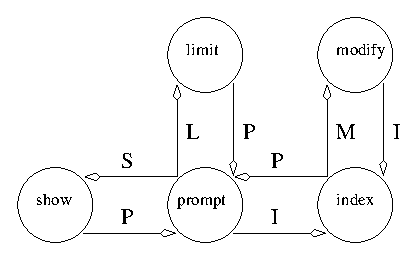
\includegraphics{../Fig8/Behavior}}
\caption{A state diagram describing the behavior of the Light Show circuit.}
\label{fig:LSbehavior}
\end{figure}

The Light Show circuit changes state when the users presses a key on 
the keyboard. For example, pressing ``M" while in the {\bf index } state causes 
the circuit to transition into the {\bf modify state}. The behavior of the 
Light Show circuit in each of its states is described in 
Table~\ref{table:LSbehavior}.

\begin{table}
\begin{tabular}{l|p{0.5in}|p{0.5in}|p{2.0in}}
{\bf State }	& LED bar graph	& 7-segment	& Behavior 				\\ \hline \hline
{\bf reset }	& blank		& blank		& All sequential elements are reset 	\\ \hline
{\bf prompt }	& blank		& ``P"		& Waiting for user input		\\ \hline
{\bf limit }	& blank		& current limit	& The number of frames in the light show is called 
	the limit. If the user enters a hex value between 0-F it is stored as the new limit. \\  \hline
{\bf index }	& current frame	& current index	& Each frame in the show has an index which defines 
	its position in the show. If the user enters a hex value between 0-F, this frame will 
	be edited in the {\bf modify } state. 						\\ \hline
{\bf modify }	& current frame	& current index	& Each frame has eight bits which specify the state of 
	the 8 LEDs on the bar graph.  These bits are toggled by pressing the corresponding 
	key. For example, if LED 5 is on, pressing ``5", causes LED 5 
	to go off.								\\ \hline
{\bf show }	& cycle through frames & current index & Consecutive frames are displayed on the 
	LED bar graph at around 4Hz. After the last frame is displayed, the circuit loops 
	back to the 0th frame. 							\\ 
\end{tabular}
\caption{The behavior of the Light Show circuit in each of its states.}
\label{table:LSbehavior}
\end{table}

The algorithm for the light show circuit continually scans the busy signal 
and the keyboard scan code.  When the user presses either a ``L", 
``I", or ``S", 
the algorithm drops into one of the subfunctions described in 
Table~\ref{table:LSbehavior}.  Assume the Light Show circuit is
clocked at 16MHz.  The clock rate is needed in order to create a delay of
0.25 seconds required to pace the frames during the show phase.  

\pagebreak
\begin{verbatim}
1.  while(1) {
2.      HexDisplay = "P"
3.      if (!busy and IsL(ScanCode)) {
4.          while (!busy' and !IsP(ScanCode)) {
5.             HexDisplay = Hex2Seven(limit);
6.             BarGraph = 0x00;
7.             if (!busy and IsHex(ScanCode)) {
8.                  limit = Scan2Hex(ScanCode);
9.                  while(!busy);
10.     }   }  }

11.     if (!busy and IsI(ScanCode)) {
12.         while (busy or !IsP(ScanCode)) {
13.             HexDisplay = Hex2Seven(index);
14.             if (!busy and IsHex(ScanCode)) {
15.                index = Scan2Hex(ScanCode);
16.                 while(!busy);
17.             }

18.             if (!busy and IsM(ScanCode)) {
19.                 while (busy or !IsI(ScanCode)) {
20.                     HexDisplay = Hex2Seven(index);
21.                     BarGraph = RAM[index];
22             	        while(!busy);
23             	        while(busy);
24.                     if (!busy and IsOct(ScanCode)) {
25.                         RAM[index] = Flip(IsOct(ScanCode),RAM[index]);
26.     }   }   }   }   }

27.     if (!busy and IsS(ScanCode)) {
28.	    index = 0;
29.         while(!busy and !IsP(ScanCode)) {
30.             BarGraph = RAM[index];
31.             HexDisplay = Hex2Seven(index);
32.             for (timer=0; timer<2^22; timer++);
33.             index += 1;
34.             if (index == limit) index=0;
35.  }  }   
\end{verbatim}

\begin{landscape}
\begin{figure}[ht]
\center{\scalebox{0.9}{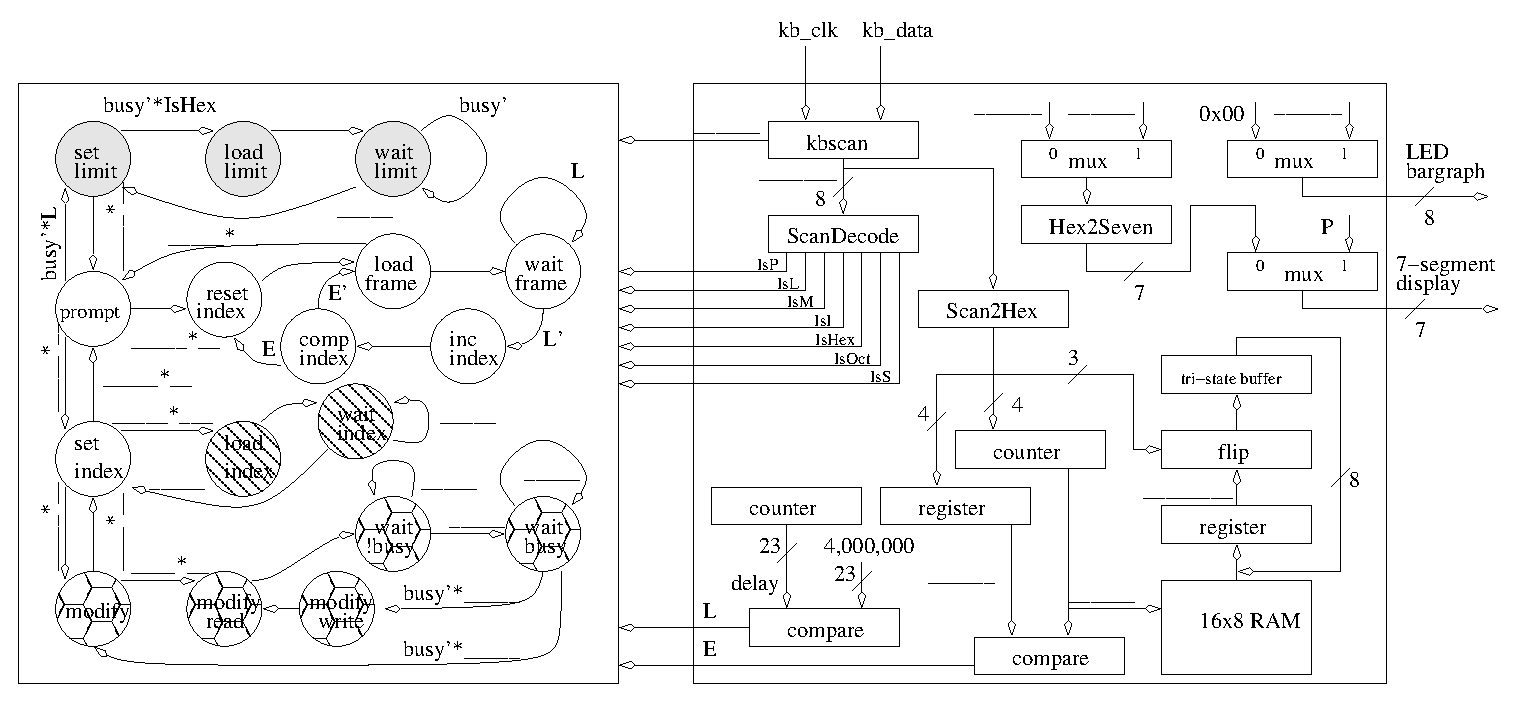
\includegraphics{./LightShowCir-hand}}}
\caption{The datapath and control for the Light show circuit.}
\label{fig:LightShowCir}
\end{figure}


\begin{table}
{\small
\begin{tabular}{c||c|c|c|c|c|c|c|c|c|c|c}
{\bf State } 	& bar & 7-seg & hex & index & delay & limit    & bargraph & CS & R/W' & tsb & flip \\  
	& mux & mux   & mux & count & count & register & register &       &       & &      \\  \hline \hline
	& 0 0x00 & 0 index & 0 7-seg & 00 hold & 00 hold & 0 hold & 0 hold & 0 off & 0 write & 0 tri & 0 pass \\ 
	& 1 bar	& 1 limit & 1 ``P"& 01 cnt & 01 cnt & 1 load &    1 load & 1 on    &  1 read & 1 pass & 1 flip \\
	& 	&     &     & 10 load & 10 load & & & & & \\
	& 	&     &	    & 11 reset	& 11 reset & & & & \\ \hline \hline
{\bf prompt } 	 & 	  &	  &	  &	   &	   &	  &	  &	  &   &	  &   \\ \hline
{\bf set limit }  & 	  &	  &	  &	   &	   &	  &	  &	  &   &	  &   \\ \hline
{\bf load limit } &	  &	  &	  &	   &	   &	  &	  &	  &   &	  &   \\ \hline
{\bf waitlimit } &	  &	  &	  &	   &	   &	  &	  &	  &   &	  &   \\ \hline
{\bf reset inde  } &	  &	  & 	  &	   &	   &	  &	  &	  &   &	  &   \\ \hline
{\bf load frame } &	  &	  &	  &	   &	   &	  &	  &	  &   &   &   \\ \hline
{\bf wait frame } &	  &	  &	  &	   &	   &	  &	  &	  &   &	  &   \\ \hline
{\bf inc index } &	  &	  &	  &	   &	   &	  &	  &	  &   &	  &   \\ \hline
{\bf comp index } &	  &	  &	  &	   &	   &	  &	  &	  &   &	  &   \\ \hline
{\bf set index } &	  &	  &	  &	   & 	   &	  & 	  &	  &   &	  &   \\ \hline
{\bf load index } &	  &	  & 	  &	   &	   &	  &	  &	  &   &   &   \\ \hline
{\bf wait index } &	  &	  &	  &	   &	   &	  &	  &	  &   &	  &   \\ \hline
{\bf modify	} &	  &	  &	  &	   &	   &	  &	  &	  &   &	  &   \\ \hline
{\bf modify read} &	  &	  &	  &	   &	   &	  &	  &	  &   &	  &   \\ \hline
{\bf modify write } &	  &	  &	  &	   &	   &	  &	  & 	  &   &	  &   \\ \hline
{\bf wait !busy } &	  &	  &	  &	   &	   &	  &	  &	  &   &	  &   \\ \hline
{\bf wait busy } &	  &	  &	  &	   &	   &	  &	  &	  &   &	  &   \\ 
\end{tabular} 
}
\caption{The control word for the LightShow circuit and its value for each state.}
\label{table:LightShow}
\end{table}

\end{landscape}

\end{document}

